\documentclass[12pt]{article}
\usepackage{indentfirst}
\usepackage{arabtex}
\usepackage{amssymb}
\usepackage{amsmath,amsthm}
\usepackage{color, xcolor}
\usepackage[ruled,vlined]{algorithm2e}
\usepackage{graphicx}
\usepackage{natbib}
\usepackage{url}
\usepackage{authblk}


\usepackage{tikz-qtree}
\usetikzlibrary{calc}
\usetikzlibrary{shapes,arrows,chains}
\usetikzlibrary{automata,positioning}
\tikzset{edge from parent/.append style={<-}}
\tikzstyle{sn}=[circle, draw, align=center, fill=white!50, inner sep=0pt, minimum size=0.6cm]

\tikzstyle{kn}=[circle, draw, align=center, fill=white!50, inner sep=0pt,
minimum size=1.6cm]

\tikzstyle{fsn}=[circle, draw, fill=blue!30, inner sep=0pt, minimum size=0.6cm]

\newtheorem{theorem}{Theorem}
\newtheorem{definition}{Definition}
\newtheorem{proposition}{Proposition}
\newtheorem{corollary}{Corollary}
\newtheorem{claim}{Claim}
\newtheorem{lemma}{Lemma}
\newtheorem{note}{Note}
\newtheorem{open}{Open}
\newtheorem{example}{Example}
\newtheorem{conjecture}{Conjecture}
\newtheorem{observation}{Observation}
\begin{document}
	\pagestyle{empty}

	\title{Implement Liquid Democracy on Ethereum: A Fast Algorithm for Realtime Self-tally Voting System}
\author[1]{Xuepeng Fan \thanks{xuepeng.fan@asresearch.io}}
\author[2]{Peng Li \thanks{pengli@u-aizu.ac.jp}}
\author[1]{Yulong Zeng \thanks{yulong.zeng@asresearch.io}}
\author[2]{Xiaoping Zhou \thanks{d8211110@u-aizu.ac.jp}}
\affil[1]{Autonomous System Research}
\affil[2]{The University of Aizu}

	%{\author{Xuepeng Fan\\ASResearch\\xuepeng.fan@asreserach.io}
	%\author{Peng Li\\The University of Aizu\\pengli@u-aizu.ac.jp}
	%\author{Yulong Zeng\\ASResearch\\yulong.zeng@asreserach.io}
	%\author{Xiaoping Zhou\\The University of Aizu\\d8211110@u-aizu.ac.jp}}
\maketitle
\begin{abstract}
	We study the liquid democracy problem, where each voter can either directly vote to a candidate or delegate his voting power to a proxy. We consider the implementation of liquid democracy on the blockchain through Ethereum smart contract and to be compatible with the realtime self-tallying property, where the contract itself can record  ballots and update voting status upon receiving each voting massage.  A challenge comes due to the gas fee limitation of Ethereum mainnet, that the number of instruction for processing a voting massage can not exceed a certain amount, which restrict the application scenario with respect to algorithms whose time complexity is linear to the number of voters. We propose a fast algorithm to overcome the challenge, such that i) shifts the on-chain initialization to off-chain and ii) the on-chain complexity for processing each voting massage is $O(\log n)$, where $n$ is the number of voters. Experimental results show that our algorithm supports $n=1000000$ in the worst case for liquid democracy on Ethereum mainnet.
\end{abstract}

\section{Problem Description}
Suppose there are $n$ voters, each voter has a certain amount of voting power $a[i],i=1,2,...,n$.

The liquid democracy refers that, each voter (called delegator) can delegate all his voting power to another voter (called delegatee), and his degegatee can further delegate all those voting power to another delegatee. Whenever a delegatee votes to a candidate, by default, all his delegators' (including multi-level) voting powers are also cast to that candidate.

We use a (direct) graph $G=(V,E)$ to represent the delegate relationship among
voters, where each note represents a voter, and a direct edge $(u,v)$
represents that voter $v$ delegates to voter $u$. Since by default there is no
loop in $G$, thus $G$ is a forest (multiple trees). For convenience, in the
case where there are more than one connect branch, we add a virtual node that
is pointed by the root of each branch. So $G$ is transferred to tree $T$, as
Figure~\ref{fig:1}.

That is, there are 12 voters, each node's  (voter) parent represents its
delegatee. As an example, now we  suppose $a[i]=i$. At the beginning, nobody
votes. When voter 1 votes for candidate $A$ (as the first voter), $A$ obtains
$1+2+...+12=78$ votes.

Meanwhile liquid democracy allows voters to change their votes when they are unsatisfied with the voting results of delegatees (including multilevel). Correspondingly, their delegatees' voting powers decrease.

As Figure~\ref{fig:1}, after voter 1 votes, suppose voter 5 (as the second
voter) votes for candidate $B$. Then $B$ obtains $6+5=11$ votes. $A$'s vote
decreases by 11, turning into 67.

Suppose further, voter 3 (the third voter) votes for candidate $C$, then $C$
obtains $3+4+7+8=22$ votes, $A$'s  vote become 45, and $B$'s vote is still 11.

\begin{figure*}
  \centering
	\label{fig:1}
	%\includegraphics[width=0.6\textwidth]{1.png}
	%\includegraphics[width=0.6\textwidth]{2.png}
	%
  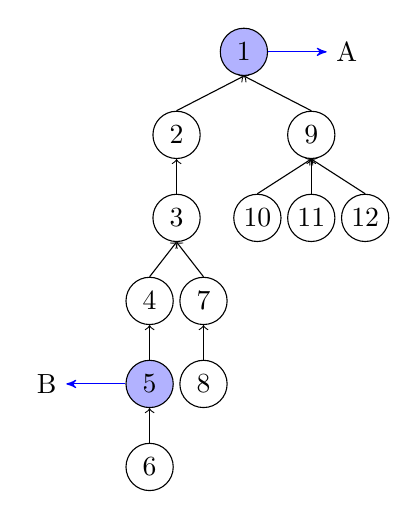
\begin{tikzpicture}
%\tikzset{grow'=right,level distance=32pt}
%\tikzset{execute at begin node=\strut}
%\tikzset{every tree node/.style={anchor=base west}}
\Tree
[.\node[fsn](n1){1};
  [.\node[sn]{2};
   [.\node[sn]{3};
    [.\node[sn]{4};
     [.\node[fsn](n5){5};
      [.\node[sn]{6};]]]
    [.\node[sn]{7};
     [.\node[sn](n8){8};]]] ]
  [.\node[sn]{9};
   [.\node[sn]{10};]
   [.\node[sn]{11};]
   [.\node[sn]{12};]]
]
\node (a) at ($(n1.east) + (1, 0)$) {A};
\node (b) at ($(n5.west) + (-1, 0)$) {B};
\draw [->, >=stealth', color=blue] (n1) -- (a);
\draw [->, >=stealth', color=blue] (n5) -- (b);

\end{tikzpicture}

	\caption{Tree $T$. We ignore the virtual node with index 0 here.}
\end{figure*}
\subsection{Goal}
Input $n<10000000,a[i],T$. Each time input a voter and a candidate that he votes, output the current voting state of all candidates (with time complexity $O(\log n)$).

Example:

\begin{tabular}{|c|c|}
input & output \\
1 A			&		A 78 B 0 C 0
\\
5 B			&		A 67 B 11 C 0
\\
3 C			&		A 45 B 11 C 22
\end{tabular}



\section{Related Work}
1. block chain and e-voting. 

2. about liquid demo: [liquid democracy journal]: total overview

[Liquid Democracy: Potentials, Problems, and Perspectives]

Arxiv:[Binary Voting with Delegable Proxy: An Analysis of Liquid Democracy ]

To the best of our knowledge our paper is the first ...

[Google vote and liquid feedback]
--3.about shifting from on-chain to off-chain 
\section{Preliminary}
\subsection{Problem Description}
Suppose there are $n$ voters, indexed by numbers $1,2,...,n$, and $m$ candidates, indexed by capital letters $A,B,C,...$. We separate the liquid democracy  problem into three periods:
\begin{itemize}
	\item \textbf{Spare period} During spare period, no voting  is hold. Each voter can arbitrarily delegate, undelegate and change delegate, by sending a massage (transaction) to the blockchain, which is stored in the delegate contract. Each voter is allowed to appoint at most one delegate. 
	\item \textbf{Prepare period}
	In prepare period, a specific voting is to be hold. The holder needs to deploy the voting contract and the delegate graph and each voters voting powers need to be constructed. In the following example we regard the delegate graph as input,  while in the next section we will show how the voting powers are determined and how to handle the case where there is a loop in the delegate graph. %and return a no-loop graph.
	\item \textbf{Voting period} After the voting begins, each voter can directly vote to a candidate by sending a voting message, with all his delegators' voting powers also cast to that candidate (which may also reduce the vote of the candidate that his delegate votes). The on-chain voting status are updated for each voting message and need to be displayed. For convenience, we assume that each voter can only vote once during each voting activity, while our algorithm also fits for the case where each voter can change his vote. A voter's delegate is not allowed to change during voting period.
\end{itemize}
It is notable that, although our algorithm does not allow voters to change their delegates during the voting period, they can accomplish the same thing by casting a direct vote.  Changing delegate to a voter that has voted is equivalent to casting a direct vote and changing delegate to a voter that has not voted is rare in practice. Actually, a voter want to change his delegate during the voting period usually because he dislikes the way his delegate votes, which means that he has a better candidate in mind and can vote by himself.

The following example illustrates how voting status changes upon receiving voting massages during voting  period.
%Suppose there are $n$ voters, each voter has a certain amount of voting power $a[i],i=1,2,...,n$.
%The liquid democracy refers that, each voter (called delegator) can delegate all his voting power to another voter (called delegatee), and his degegatee can further delegate all those voting power to another delegatee. Whenever a delegatee votes to a candidate, by default, all his delegators' (including multi-level) voting powers are also cast to that candidate.
 Suppose a (direct, no-loop) delegate graph $G=(V,E)$ is given, where each node represents a voter, and a direct edge $(u,v)$ represents that voter $v$ delegates to voter $u$. We will use terms ``voter" and ``node" interchangeably in the following of this paper.  Since by assumption there is no
loop in $G$, thus $G$ is a forest (multiple trees). For convenience, we add a virtual node (indexed 0) that
is pointed by the root of each connected branch. So $G$ is transferred to tree $T$, as
Figure~\ref{fig:1}. That is, there are 12 voters. We further assume that each voter's voting power equals to his index. 

\begin{itemize}
\item At the beginning, nobody
votes. When voter 1 votes for candidate $A$ (as the first voter), $A$ obtains
$1+2+...+12=78$ votes.

\item After voter 1 votes, suppose voter 5 (as the second
voter) votes for candidate $B$. Then $B$ obtains $6+5=11$ votes. $A$'s vote
decreases by 11, turning into 67.

\item Further, voter 3 (as the third voter) votes for candidate $C$, then $C$
obtains $3+4+7+8=22$ votes, $A$'s vote becomes 45, and $B$'s vote is still 11.
\end{itemize}

\begin{figure*}
  \centering
  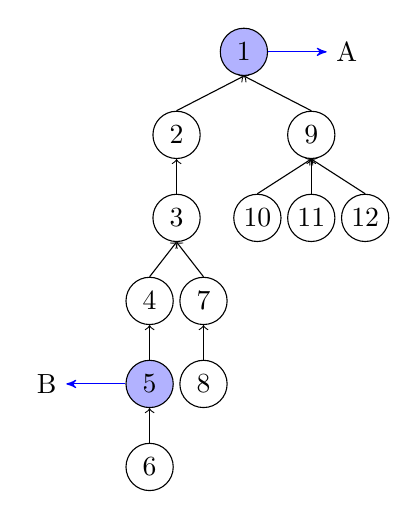
\begin{tikzpicture}
%\tikzset{grow'=right,level distance=32pt}
%\tikzset{execute at begin node=\strut}
%\tikzset{every tree node/.style={anchor=base west}}
\Tree
[.\node[fsn](n1){1};
  [.\node[sn]{2};
   [.\node[sn]{3};
    [.\node[sn]{4};
     [.\node[fsn](n5){5};
      [.\node[sn]{6};]]]
    [.\node[sn]{7};
     [.\node[sn](n8){8};]]] ]
  [.\node[sn]{9};
   [.\node[sn]{10};]
   [.\node[sn]{11};]
   [.\node[sn]{12};]]
]
\node (a) at ($(n1.east) + (1, 0)$) {A};
\node (b) at ($(n5.west) + (-1, 0)$) {B};
\draw [->, >=stealth', color=blue] (n1) -- (a);
\draw [->, >=stealth', color=blue] (n5) -- (b);

\end{tikzpicture}

  	\caption{Tree $T$. We ignore the virtual node with index 0 here.}
  		\label{fig:1}
\end{figure*}
\textbf{Goal}:
For each voting massage, display the votes of all candidates. (Suppose $m<100$)

\begin{tabular}{|c|c|}
input & output \\
1 A			&		A 78 B 0 C 0
\\
5 B			&		A 67 B 11 C 0
\\
3 C			&		A 45 B 11 C 22
\end{tabular}
\subsection{Blockchain and Smart Contract}
The smart contract of Ethereum supports Turing-complete programming language, which is deployed on the blockchain \cite{bocek2018smart}. Users invoke a smart contract by sending a transaction to the smart contract's address, which contains additional information including the gas fee of the transaction and other incoming parameters, which would further be included in a block. As shown in section 1, the gas fee of a valid transaction are limited by the fixed parameter block\_gas\_limit, so that the number of instructions of the smart contract are also bounded. That is the so-called "on-chain" time complexity. In this paper, we use ``voting massage" to represent the transaction that invokes the voting contract, whose on-chain time complexity are required to be sub-linear to the number of voters.  Ethereum clients obtain latest on-chain data through P2P network and implement smart contracts locally through Etheruem virtual machine (EVM). Thus, the space limitation of a smart contract only depends on Ethereum nodes' (clients) local storage, which is not an issue in this paper.

It is important to distinguish on-chain smart contract and (open source) cloud computation. The later is still realized by centralized servers, which can not guarantee the codes are correctly executed, while in Ethereum, there is no "center" for executing smart contract: they are executed by every Ethereum node, which is reliable as long as the majority of nodes are honest.

\subsection{Merkel Tree}
The Merkel Tree is a common used method for store and verifying on-chain data. One of the key tools is the hash function, $h()$, which is (cryptographically) hard to find collisions and for inverse computation (In Ethereum, SHA3-256 is used). The Merkel tree is a full binary tree, where each leaf node stores the hash value of data to be stored (see Figure \ref{fig:merkel}). The value of an intermediate node is the hash value of the combination of its two children. 
\begin{figure*}
	\centering
	\label{fig:merkel}
	\includegraphics[width=1.1\textwidth]{merkel.png}
	%\includegraphics[width=0.6\textwidth]{2.png}
	\caption{Merkel tree, where $h_{A/B/C/D}$ refers to the hash value of data $A/B/C/D$. The black nodes represent the Merkel path of data $A$}
\end{figure*}

The use of Merkel tree is that, the blockchain only need to store the root of the Merkel tree. In order to proof that a data (say data $A$ in the Figure \ref{fig:merkel})belongs to the Merkel tree, $A$ along with its Merkel path (also called Merkel Proof) are required:

\textbf{Merkel path}, which is defined to be a sequence of nodes in the Merkel tree that corresponds to brother of each node on path from  $A$'s leaf node to the root. For example, data $A$'s Merkel path is $(h_B,h_{CD})$. A leaf node together with its correct Merkel path can recover the root of the Merkel tree (called Merkel root). The length of the Merkel path and the time complexity for recovering the Merkel root are all logarithmic to the number of leaf nodes of the Merkel tree. The one-wayness of the hash function guarantees that it is hard to construct a correct Merkel path for any data that does not belong to any leaf nodes of the Merkel tree.
\subsection{Interval Tree}
Interval tree is also a binary tree, where each node represents a interval and the interval of a parent node is uniformly distributed to its two child nodes, until the interval becomes a singular, to be a leaf node. 
\begin{figure}
	\centering
	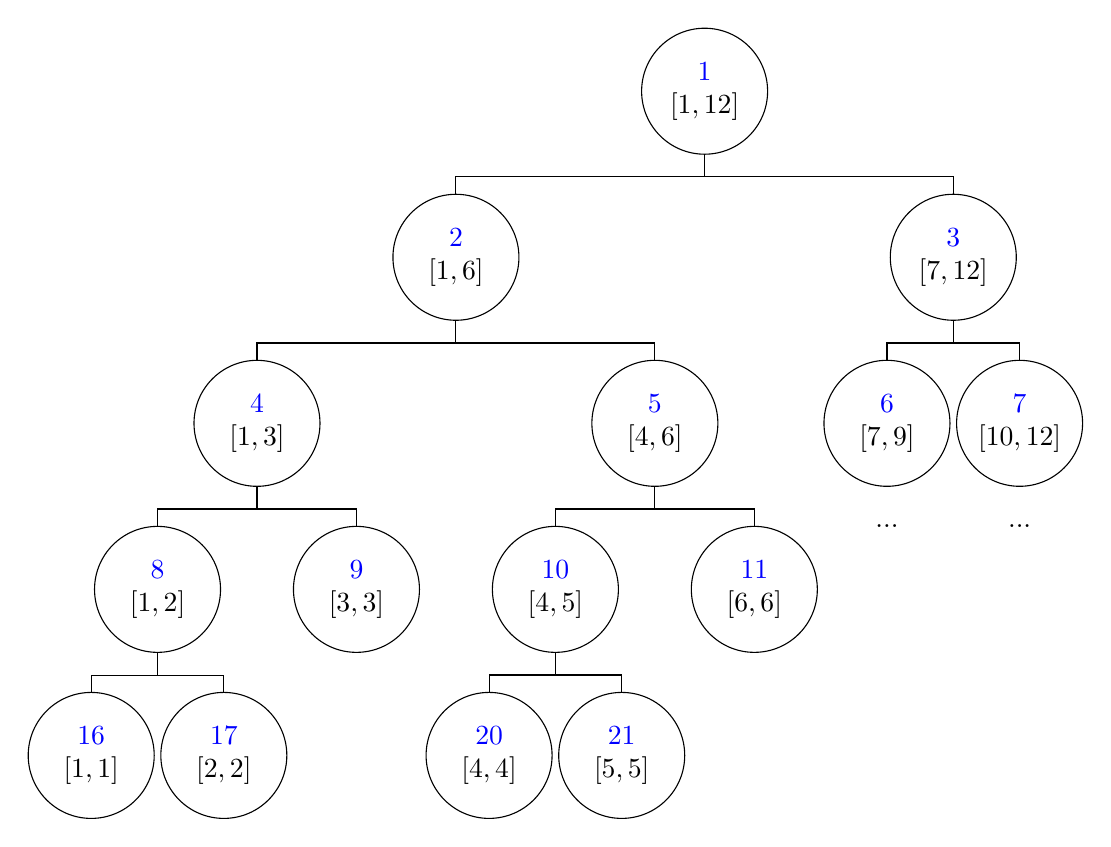
\begin{tikzpicture}[level distance=60pt]
\tikzset{edge from parent/.style=
{draw,
edge from parent path={(\tikzparentnode.south)
-- +(0,-8pt)
-| (\tikzchildnode)}}}
%\tikzset{grow'=right,level distance=32pt}
%\tikzset{execute at begin node=\strut}
%\tikzset{every tree node/.style={anchor=base west}}
\Tree
[.\node[kn](n1){{\color{blue}1}\\$[1,12]$};
  [.\node[kn]{{\color{blue}2}\\$[1,6]$};
   [.\node[kn]{{\color{blue}4}\\$[1,3]$};
    [.\node[kn]{{\color{blue}8}\\$[1,2]$};
     [.\node[kn]{{\color{blue}16}\\$[1,1]$};]
     [.\node[kn]{{\color{blue}17}\\$[2,2]$};]
    ]
    [.\node[kn]{{\color{blue}9}\\$[3,3]$};]
   ]
   [.\node[kn]{{\color{blue}5}\\$[4,6]$};
    [.\node[kn]{{\color{blue}10}\\$[4,5]$};
     [.\node[kn]{{\color{blue}20}\\$[4,4]$};]
     [.\node[kn]{{\color{blue}21}\\$[5,5]$};]
    ]
    [.\node[kn]{{\color{blue}11}\\$[6,6]$};]
   ]
  ]
  [.\node[kn]{{\color{blue}3}\\$[7,12]$};
   [.\node[kn](n6){{\color{blue}6}\\$[7,9]$};]
   [.\node[kn](n7){{\color{blue}7}\\$[10,12]$};]]
]

\node (a) at ($(n6.south) + (0, -0.5)$) {...};
\node (b) at ($(n7.south) + (0, -0.5)$) {...};
\end{tikzpicture}

	\caption{The interval tree of all nodes}
				\label{fig:interval}
\end{figure}
See Figure \ref{fig:interval} for the interval tree of the 12 nodes in Figure \ref{fig:1}. The root are indexed 1 and for node $k$, its child nodes are indexed $2k,2k+1$ respectively. Note that, although some indexes, e.g. 18,19 in Figure \ref{fig:merkel}, does not exist, the space is still used. 

Interval tree is usually used for maintaining an array where the operations are aiming at a successive interval. Given the interval to be updated, the execution begins at the root node, then the interval are separated to one or two sub-intervals. which are recursively executed at the child notes, guaranteeing that the sub-intervals to be update belongs to interval of current node. The recursion ends when the interval to be update equals to the interval of current node. For example, when interval 
[4,8] is to be update, beginning at the root, it separates to [4,6] and [7,8], which are executed at note 2 and 3 respectively. The recursion ends at node 5 and node 12 (which are omitted in Figure \ref{fig:interval}).

Interval tree support find and update operation. For update operation, usually not every leaf node is updated since the update information may stop at an intermediate node, recorded as lazy-tag, which means that it is temporarily suspended and will be executed in subsequent operations. Find operations need to be executed recursively starting from the root, and trigger the pass-down operation of all lazy-tags until the leaf node is reached. The complexity is $O(\log n)$ with respect to interval tree for both operations. We refer \cite{mulmuley1994computational}, Chapter 10.1 to readers for more detail.



\section{Algorithm}
\subsection{Overview}
Our algorithm fully solves the liquid democracy problem. Compare to other algorithms discussed in the forum\footnote{https://forum.aragon.org/t/open-challenges-for-on-chain-liquid-democracy/161}, it has the following feature:
\begin{itemize}
	\item Our algorithm supports the tree with any structure, from a chain to star graph, without any restriction to max-depth.
	\item Our algorithm supports the realtime display of voting state (all candidates' votes), with on-chain time complexity $O(\log n)$
	\item Our algorithm requires on-chain space complexity $O(n)$ and off-chain time-complexity $O(n)$.
\end{itemize}
The core of the liquid democracy problem is the state transition when a voter votes. We record ``lost voting power" for any node, representing the total voting power that its child nodes have cast, initialing 0.  One of the key point is that, when a voter votes, his effective votes is his total voting power minus his lost voting power, and the voting operation \textbf{only affects the lost voting power of nodes on the path from its direct parent to its nearest parent that has already cast a vote (we call nearest voted parent).} Actually, the lost voting power of nodes on the path should increases by the amount of the voters effective votes. We use a data structure called interval tree to update.

Our algorithm consists of the following three parts.
\begin{itemize}
	\item Initiation: including computing the total voting power of all nodes, getting the nodes' numbers in the pre-order sequence and so on. Require time complexity $O(n)$
	\item For each voting operation, finding the voter's nearest voted parent.
	\item For each voting operation, maintain nodes' lost voting powers.
\end{itemize}

We have the following variables:
\begin{itemize}
	\item $T$: The liquid democracy tree, regard as input.
	\item $n$: Number of nodes
	\item $node.index$: Index of the node in the pre-order sequence.
	\item $node.address$: The address of each node.
	\item $b[n]$: Mapping from index to node.
	\item $nearestparent[n]$: Nearest voted parent of the nodes, with the index in the pre-order sequence.
	\item $node.endpoint$: Right endpoint of node's interval in the pre-order sequence.
	\item $node.votingpower$: Nodes total voting power (including its delegators').
	\item $node.candidate$: Recording the candidate that the voter votes.
	\item $v[]$: Recording the votes of candidates.
\end{itemize}
%Note that the initiation part only needs to be executed once, it can be realized by off-chain code, and then update to the on-chain contract through merkel root. To be straight, we first introduce the part 2 and 3 and suppose $O(n)$ initiation is allowed.

\subsection{Initiation}
It is not allowed to do on-chain initiation due to the $O(n)$ complexity, we
can realize it through merkel root. The initiation process is done by the vote
creator.

We first assign a index in the pre-order sequence for each node in the initiation part. Note that the pre-order sequence has the following property
\begin{enumerate}
	\item A node always has index smaller than that of its child nodes.
    \item For each nodes, all its child notes continuously appear after it in the pre-order sequence.
	\item If a node's nearest voted parent is $x$, all its child nodes' nearest voted parent is $x$ or a node with index larger than $x$.
\end{enumerate}
\begin{algorithm}
	\label{alg:preorder}
	\textbf{Procedure} $Preorder(Node~root)$;
	\hrule
	$n \leftarrow n+1$\;
	$m \leftarrow m+1$
	$root.leftbracket \leftarrow m${\color{gray}//For bracket sequence}\;
	%$n_0 \leftarrow n$\;
	%$S[n] \leftarrow root$\;
	$root.index \leftarrow n$\;
	$b[n]=root$\;
	\For{$node$ in $root$'s direct child}
	{
		$Preorder(node)$
	}
	$root.endpoint \leftarrow n$\;
	$m \leftarrow m+1$\;
	$root.rightbracket \leftarrow m${\color{gray}//For bracket sequence}\;
\end{algorithm}
The preorder function is to get each node's index and corresponding interval for child nodes, in the preorder sequence.

The next step is to create a Merkel tree, and each leaf node is computed like
this:
\[
  hash(node.address, node.endpoint, node.index).
\]
\noindent The vote creator need to pass the Merkel root as parameter when
creating the vote. And the Merkel root is stored on-chain.


\subsection{Vote}
For each voter, they need to get their information, like $endpoint$ and $index$. They can achieve
this by either contact the vote creator (through a web page) or do the
initiation process themselves. Each
voter needs to provide their information and also a Merkel proof when casting their vote. And
the contract determines whether the provided information is correct since the
Merkel root is already on-chain.

We then introduce the main algorithm, Algorithm~\ref{alg:vote}. Note this
algorithm is on-chain. To run this algorithm, the contract need to initiate several arrays (
\texttt{mapping} in Solidity). Although the arrays' sizes are $O(n)$, they can
be initiate with 0, which is the default value on Solidity.

\begin{algorithm}
	\caption{Vote}%算法名字
  \KwIn{$node$: voter}
  \KwIn{$proof$: voter's Merkel proof}
	\hrule
    $h \leftarrow hash(node.address, node.index, node.endpoint);$

    \If {not check(RootHash, proof, h)}{
      \Return ;
    }
		$update2(node.leftbracket,node.leftbracket,1,2n,1,0)${\color{gray}
			//Find the value of node's leftbracket}\;
		$update2(node.rightbracket,node.rightbracket,1,2n,1,0)${\color{gray}
			//Find the value of node's rightbracket}\;
		$int~t=node.votingpower-lazy2[node.leftbracket]+lazy2[node.rightbracket]$\;
		$C[node.candidate]+=t$\;
		$update1(node.index,node.index,1,n,1,0)${\color{gray}
			\\//Find the the node's nearest parent}\;
		$Node~parent = b[nearestparent[node.nunmber]]$\;
		$C[parent.candndate]-=t$\;
		$update1(node.index+1,node.endpoint,1,n,1,node.index)${\color{gray}
			\\//Update the first interval tree}\;
		$update2(parent.leftbracket,node.leftbracket-1,1,2n,1,t)${\color{gray}
			\\//Update the second interval tree}\;
		Output $C[]$
  \label{alg:vote}
\end{algorithm}
Also note that $RootHash$ is already stored on-chain.

\subsection{Finding Nearest Parent}
In this subsection we realize the function that finding the a node's nearest parent.

\begin{figure}
	\centering
	%\includegraphics[width=0.6\textwidth]{3.png}
	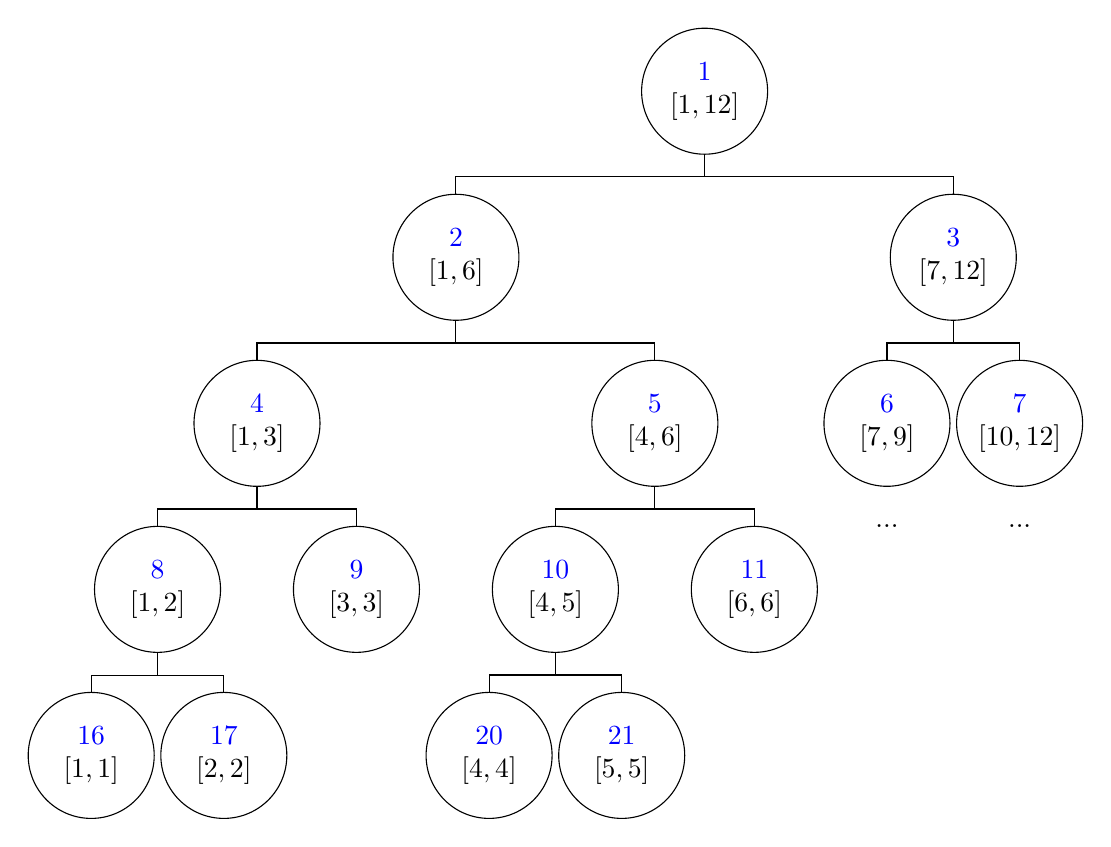
\begin{tikzpicture}[level distance=60pt]
\tikzset{edge from parent/.style=
{draw,
edge from parent path={(\tikzparentnode.south)
-- +(0,-8pt)
-| (\tikzchildnode)}}}
%\tikzset{grow'=right,level distance=32pt}
%\tikzset{execute at begin node=\strut}
%\tikzset{every tree node/.style={anchor=base west}}
\Tree
[.\node[kn](n1){{\color{blue}1}\\$[1,12]$};
  [.\node[kn]{{\color{blue}2}\\$[1,6]$};
   [.\node[kn]{{\color{blue}4}\\$[1,3]$};
    [.\node[kn]{{\color{blue}8}\\$[1,2]$};
     [.\node[kn]{{\color{blue}16}\\$[1,1]$};]
     [.\node[kn]{{\color{blue}17}\\$[2,2]$};]
    ]
    [.\node[kn]{{\color{blue}9}\\$[3,3]$};]
   ]
   [.\node[kn]{{\color{blue}5}\\$[4,6]$};
    [.\node[kn]{{\color{blue}10}\\$[4,5]$};
     [.\node[kn]{{\color{blue}20}\\$[4,4]$};]
     [.\node[kn]{{\color{blue}21}\\$[5,5]$};]
    ]
    [.\node[kn]{{\color{blue}11}\\$[6,6]$};]
   ]
  ]
  [.\node[kn]{{\color{blue}3}\\$[7,12]$};
   [.\node[kn](n6){{\color{blue}6}\\$[7,9]$};]
   [.\node[kn](n7){{\color{blue}7}\\$[10,12]$};]]
]

\node (a) at ($(n6.south) + (0, -0.5)$) {...};
\node (b) at ($(n7.south) + (0, -0.5)$) {...};
\end{tikzpicture}

	\caption{Interval tree, where the blue number in each node is the index of the node on the interval tree and the interval in each node represents the interval of the preorder sequence}
	\label{fig:3}
\end{figure}
Interval tree\footnote{\url{https://en.wikipedia.org/wiki/Interval_tree}}, is
fits for operations that aim to a continuous interval. We construct an interval
tree (Figure~\ref{fig:3}) with respect to the pre-order sequence and record each node's nearest voted parent. Each time a voter votes, we update the interval that represent the voter's child nodes in the interval tree.

We add a new global variable here.
\begin{itemize}
	\item $lazy1[2n]$: Lazy-tag in the first interval-tree\footnote{Lazy-tag is a normal operation for interval tree: when we update an interval, we can not update all the leave nodes in the interval (otherwise the time complexity is $O(n)$). Instead, we first leave the updating information to an intermediate node, that known as lazy, when next time we need to find a node included in the interval, we then sink down the lazy-tag. }
\end{itemize}

\begin{algorithm}
	\textbf{procedure} $update1(int~L,int ~R, int~l, int~r, int~k, int~v)${\color{gray}
		\\//$L,R$ are the interval for updating, and $l,r$ are node's interval,$k$ is the index of the node on interval tree, $v$ is the value for updating the interval.}
	\hrule
	\eIf {$L=l$ and $R=r$}
	{
		\If {$v>lazy1[k]$} {$lazy1[k] \leftarrow v$}
		\If {$L = R$} {$nearestparent[L] = lazy1[k]$}
		{\color{gray}
		//Recursion ends when updating interval equals to the node's interval, and then updating the value of the interval}
	}
	{
		$int~m \leftarrow (l+r)/2$\;
		\If {$lazy1[2k]<lazy[k]$} {$lazy1[2k] \leftarrow lazy1[k]$}
		\If {$lazy1[2k+1]<lazy[k]$} {$lazy1[2k+1] \leftarrow lazy1[k]${\color{gray}
			//sink down the lazy-tag}}
		\If {$L \leq m$}{$update(L,\min\{m,R\},l,m,2k,v)$}
		\If {$R>m$}{$update(\max\{m+1,L\},R,m+1,r,2k+1,v)$}
	}
\end{algorithm}
We use $update1$ to finding and update the interval tree. No extra code is needed for building the interval tree as we use $k,2k,2k+1$ to represent a node and its two children for a node in the interval tree.

The inherent property of interval tree guarantees that, there are at most two intervals in each depth that are recursively processed, so the time complexity for each updating is $O(\log n)$.

\subsection{Updating Lost Voting Power}
When a voter votes, all nodes on the path from the voter to its nearest voted parented should update their lost voting powers. See Figure \ref{fig:2}, if voter 8 votes after voter 1 votes, then path $7,3,2,1$ should be updated. However it is not a continuous interval in the pre-order sequence.
\begin{figure}
  \centering
	%\includegraphics[width=0.6\textwidth]{3.png}
  
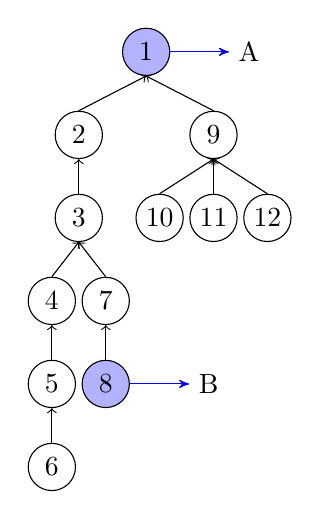
\begin{tikzpicture}
%\tikzset{grow'=right,level distance=32pt}
%\tikzset{execute at begin node=\strut}
%\tikzset{every tree node/.style={anchor=base west}}
\Tree
[.\node[fsn](n1){1};
  [.\node[sn]{2};
   [.\node[sn]{3};
    [.\node[sn]{4};
     [.\node[sn]{5};
      [.\node[sn]{6};]]]
    [.\node[sn]{7};
     [.\node[fsn](n8){8};]]] ]
  [.\node[sn]{9};
   [.\node[sn]{10};]
   [.\node[sn]{11};]
   [.\node[sn]{12};]]
]
\node (a) at ($(n1.east) + (1, 0)$) {A};
\node (b) at ($(n8.east) + (1, 0)$) {B};
\draw [->, >=stealth', color=blue] (n1) -- (a);
\draw [->, >=stealth', color=blue] (n8) -- (b);

\end{tikzpicture}

	\caption{Updating a path}
	\label{fig:2}
\end{figure}
We use the bracket sequence to handle this problem. A bracket sequence is to
record each node twice in the pre-order execution, one for enter and one for
exit, called left bracket and right bracket respectively. For Figure~\ref{fig:2}, the bracket sequence is
$$1,2,3,4,5,6,6,5,4,7,8,8,7,3,2,9,10,10,11,11,12,12,9,1$$
Let array $s[2n]$ record a value of the bracket sequence. When vote 8 votes, we let $s[1-10]+=8$, that is, the interval form node 1's left bracket to the node before node 8's left bracket.

The lost voting power of a node $u$ is $s[u.leftbracket]-s[u.rightbracket]$.

To see why, it is not hard to find that, if a node does not occur on the path we need update, it occurs twice in the interval (1-10) of the bracket sequence, say node 4,5,6. If a node is to be update, it occurs only once in the interval  (1-10) of the bracket sequence, say node 1,2,3. So from maintaining the array $s$ we can maintain each node's lost voting power. Since now the operation is an interval again, we can use another interval tree to handle it.

We add the following variables:
\begin{itemize}
%\item $s[2n]$, recording the value of the bracket sequence.
\item $lazy2[4n]$, the lazy-tag of the second interval tree.
\item $node.leftbracket,node.rightbracket$
\end{itemize}

\begin{algorithm}
	\textbf{procedure} $update2(int~L,int ~R, int~l, int~r, int~k, int~v)${\color{gray}
		\\//$L,R$ are the interval for updating, and $l,r$ are node's interval,$k$ is the index of the node on interval tree, $v$ is the value for updating the interval.}
	\hrule
	\eIf {$L=l$ and $R=r$}
	{
       $lazy2[k]+=v$
	   %\If {$L = R$} {}
	}
	{
		$int~m \leftarrow (l+r)/2$\;
		$lazy2[2k] += lazy2[k]$\;
		$lazy2[2k+1]+= lazy2[k]$\;
		$lazy2[k] \leftarrow 0$
			{\color{gray}
		//sink down the lazy-tag}\;
		\If {$L \leq m$}{$update2(L,\min\{m,R\},l,m,2k,v)$}
		\If {$R>m$}{$update2(\max\{m+1,L\},R,m+1,r,2k+1,v)$}
    }
\end{algorithm}

\section{Theorem}
In this section we prove some properties of our algorithm. We first analyze our protocol for constructing the delegate graph.
\begin{lemma}
   If a voter's delegate operation does not generate a cycle of the delegate graph (locally checked), then the corresponding edge will never be deleted. 
\end{lemma}
\begin{proof}
	Assume by contradiction that the delegate edge is deleted. By definition, there must be a cycle such that the delegate edge is the latest, which means that the cycle are generated by the appearance of the delegate edge, contradiction.
\end{proof}
It means that, if the voter follows the protocol, then his delegation are garanteed to be retained, which is benefit for him. Otherwise if he deviates (his delegation generates a cycle), his delegation may be deleted. (It is also possible to be retained, if other voters further change their delegate and remove the cycle)
\begin{lemma}
	If a voter deviates from our mechanism, by sending a delegate edge that generates a cycle, then further, this edge will not cause other voter's delegate edge to be refused if they follows the protocol.
\end{lemma}
\begin{proof}
	We call the delegate edge of the dishonest voter edge $A$. We prove that, if an edge $B$ is refused with the existence of edge $A$, then it will also be refused without the existence of edge $A$.
	
	Since $B$ is refused, it lies on a cycle which contains $A$. Since $A$ also lies on another cycle, if $A$ is delete, $B$ still lies on a cycle, and should be refused according to the protocol. The lemma is proved.
\end{proof}
The lemma shows that, even if a voter deviates from the protocol, other voters are not influenced. 

There are also sublinear-time algorithms that can judge whether a cycle is generated for a incoming delegate edge, which can be used in smart contract. However it is more complex and require more gas fee for each delegate massage. So still our protocol is recommended in practice. 

Next, we introduce our main theorem:
\begin{theorem}
	For each voting massage in liquid democracy problem, the voting status can be updated and displayed within $O(\log n)$ time complexity. Moreover, our algorithm can be deploy on the Ethereum mainnet and overcome the gas limitation, for the number of voters more than one million.
\end{theorem}
The theorem is obvious according to the properties of the tools we used. Here we illustrate some issues.
\begin{itemize}
	\item Processing a voter's voting message does not rely on the initialization data of other voters that has not voted, since our algorithm only requires the data from the nearest voted parent.
	\item The ``mapping" structure in Solidity (the coding language of Ethereum smart contract) satisfies that, the storages are allocated only if they are assigned values. For example, the storage $lazy[3]$ can be allocated without the allocation of $lazy[1]$ and $lazy[2]$. Moreover, $lazy[1]$ and $lazy[2]$ still can be visit but always returned a default value 0, which is just the requirement of our algorithm.
	\item The time complexity of update operation in interval tree is $O(\log n)$, since at each level of the interval tree, at most two intervals are at the recursive state: except for the interval tree root, there are at least one endpoints of the interval to be update are the same as the endpoints of the interval of current node. So at the next level, either there are only one interval to be executed, or there are two intervals, but one of them is identical to the interval of the next interval tree node, and the recursion ends. 
\end{itemize}
For the part of Ethereum, we leave the proof in the experiment section.
\section{Experiment}
We compare between our algorithm and traversal algorithm (implemented by ourselves) by
recording the maximum consumed gas fee. Since in practice the only requirement is that the  consumed gas fee should be strictly limited by related Ethereum parameter, we focus on extreme cases that produce the maximum consumed gas fee. 

We assume that the delegate graph is a chain, which turns out to be the extreme case of consumed gas fee. We also consider extreme cases where the voter comes from the head/tail of the chain, which is possible to produce the maximum consumed gas fee for both algorithm.

\begin{figure}[h]
\begin{minipage}[t]{0.5\textwidth}
 \begin{tikzpicture}[scale=0.6]
\begin{axis}[votegas]
\addplot  plot coordinates {
(10, 139758)
(20, 210619)
(30, 281487)
(40, 352360)
(50, 423240)
(60, 494126)
(70, 565018)
(80, 635916)
(90, 706821)
(100, 777732)
(200, 1487185)
(300, 2197263)
(400, 2907966)
(500, 3619294)
(600, 4331247)
(700, 5043826)
(800, 5757029)
(900, 6470857)
};\addplot  plot coordinates {
(10, 520250)
(20, 580441)
(30, 559707)
(40, 640301)
(50, 619823)
(60, 619695)
(70, 700354)
(80, 700354)
(90, 700418)
(100, 679812)
(200, 739737)
(300, 820587)
(400, 799789)
(500, 799917)
(600, 880448)
(700, 880384)
(800, 859906)
(900, 859906)
(1000, 859970)
(2000, 919895)
(3000, 1000554)
};\legend{traversal,fast}
  \draw [dashed] ( axis cs:0, 6750000) -- ( axis cs:3200, 6750000) node
  [near start, above] {Gas Limit};
\end{axis}
\end{tikzpicture}

  \caption{Voting by the head.}
  \label{fig:eval:root}
\end{minipage}
\begin{minipage}[t]{0.5\textwidth}
 \begin{tikzpicture}
\begin{axis}[votegas]
\addplot  plot coordinates {
(10, 103692)
(20, 134473)
(30, 165254)
(40, 196036)
(50, 226818)
(60, 257601)
(70, 288384)
(80, 319167)
(90, 349951)
(100, 380735)
(200, 688599)
(300, 996502)
(400, 1304444)
(500, 1612425)
(600, 1920444)
(700, 2228503)
(800, 2536601)
(900, 2844739)
(1000, 3152915)
(2000, 6236825)
};\addplot  plot coordinates {
(10, 536968)
(20, 613237)
(30, 595379)
(40, 689505)
(50, 666551)
(60, 671584)
(70, 760741)
(80, 765774)
(90, 763257)
(100, 742819)
(200, 819088)
(300, 913534)
(400, 895548)
(500, 898193)
(600, 989610)
(700, 992255)
(800, 971817)
(900, 966912)
(1000, 974398)
(2000, 1050794)
(3000, 1144856)
};\legend{traversal,fast}
  \draw [dashed] ( axis cs:0, 6750000) -- ( axis cs:3200, 6750000) node
  [near start, above] {Gas Limit};
\end{axis}
\end{tikzpicture}

  \caption{Voting by the tail.}
  \label{fig:eval:tail}
\end{minipage}
\end{figure}

We conduct the evaluation on Ganache, which is a
personal blockchain for Ethereum development that can be used to deploy contracts, and run tests.
Our implementation can be found here~\footnote{\url{https://github.com/freeof123/liquid-voting/tree/master/ether-eval/contracts}}.
%As there is no standard implementation for the traversal algorithm, we
%implement it by ourselves.  %Specifically, the traversal only happens when casting a vote, instead of delegating.

Our comparison is from two aspects. \begin{enumerate*}[1) ]%
  \item The voter is the \emph{head} of the delegate chain, as illustrated in
  Fig.~\ref{fig:eval:root}; \item the voter is the \emph{tail} of the delegate chain
, as shown in Fig.~\ref{fig:eval:tail}. \end{enumerate*}.
The gas limit is about 6,700,000 according to Ganache. Our
evaluation shows that \begin{itemize}
    \item the traversal algorithm performs better when the delegate chain
      is short, like smaller than 100;
    \item our algorithm significantly outperforms the traversal algorithm when
      the delegate chain is long enough;
    \item our algorithm can scale up with very limited gas increasing, while
      the traversal algorithm reaches the gas limit when the delegate chain
      grows up to 1,000.
\end{itemize}.




\section*{Acknowledgment}
We thank YingLiu from Peking University for the advising the algorithm.

\bibliographystyle{plain}
\bibliography{ref}
\end{document}
